% Created 2022-03-02 Wed 13:25
% Intended LaTeX compiler: pdflatex
\documentclass[presentation]{beamer}
\usepackage[utf8]{inputenc}
\usepackage[T1]{fontenc}
\usepackage{graphicx}
\usepackage{grffile}
\usepackage{longtable}
\usepackage{wrapfig}
\usepackage{rotating}
\usepackage[normalem]{ulem}
\usepackage{amsmath}
\usepackage{textcomp}
\usepackage{amssymb}
\usepackage{capt-of}
\usepackage{hyperref}
\mode<beamer>{\usetheme{Madrid}}
\usetheme{default}
\author{M. Falzari}
\date{\today}
\title{Disentangled Representation with Autoencoders for efficient DRL}
\hypersetup{
 pdfauthor={M. Falzari},
 pdftitle={Disentangled Representation with Autoencoders for efficient DRL},
 pdfkeywords={},
 pdfsubject={},
 pdfcreator={Emacs 27.2 (Org mode 9.4.4)},
 pdflang={English}}
\begin{document}

\maketitle
\begin{frame}[label={sec:org188aea2}]{Quick recap}
\begin{block}<1->{Dimensionality Reduction}
reduce the number of dimensions/features while maintaing the most
important information
\end{block}

\begin{block}<2->{Sparse Autoencoders}
\begin{itemize}
\item main goal is to learn f(g(x)) = x
\item g is the encoder and f is the decoder
\item g(x) = z where z \(\in\) \mathbb{R}\textsuperscript{n} and x \(\in\) \mathbb{R}\textsuperscript{m}
and n << m
\end{itemize}
\end{block}

\begin{block}<3->{Other techniques? and why Autoencoders?}
visit \url{https://172.104.159.41/thesis/summary.html}
section \alert{Line of Thoughts}
\end{block}
\end{frame}

\begin{frame}[label={sec:org63d1689}]{Sparse Autoencoders}
\begin{figure}[htbp]
\centering
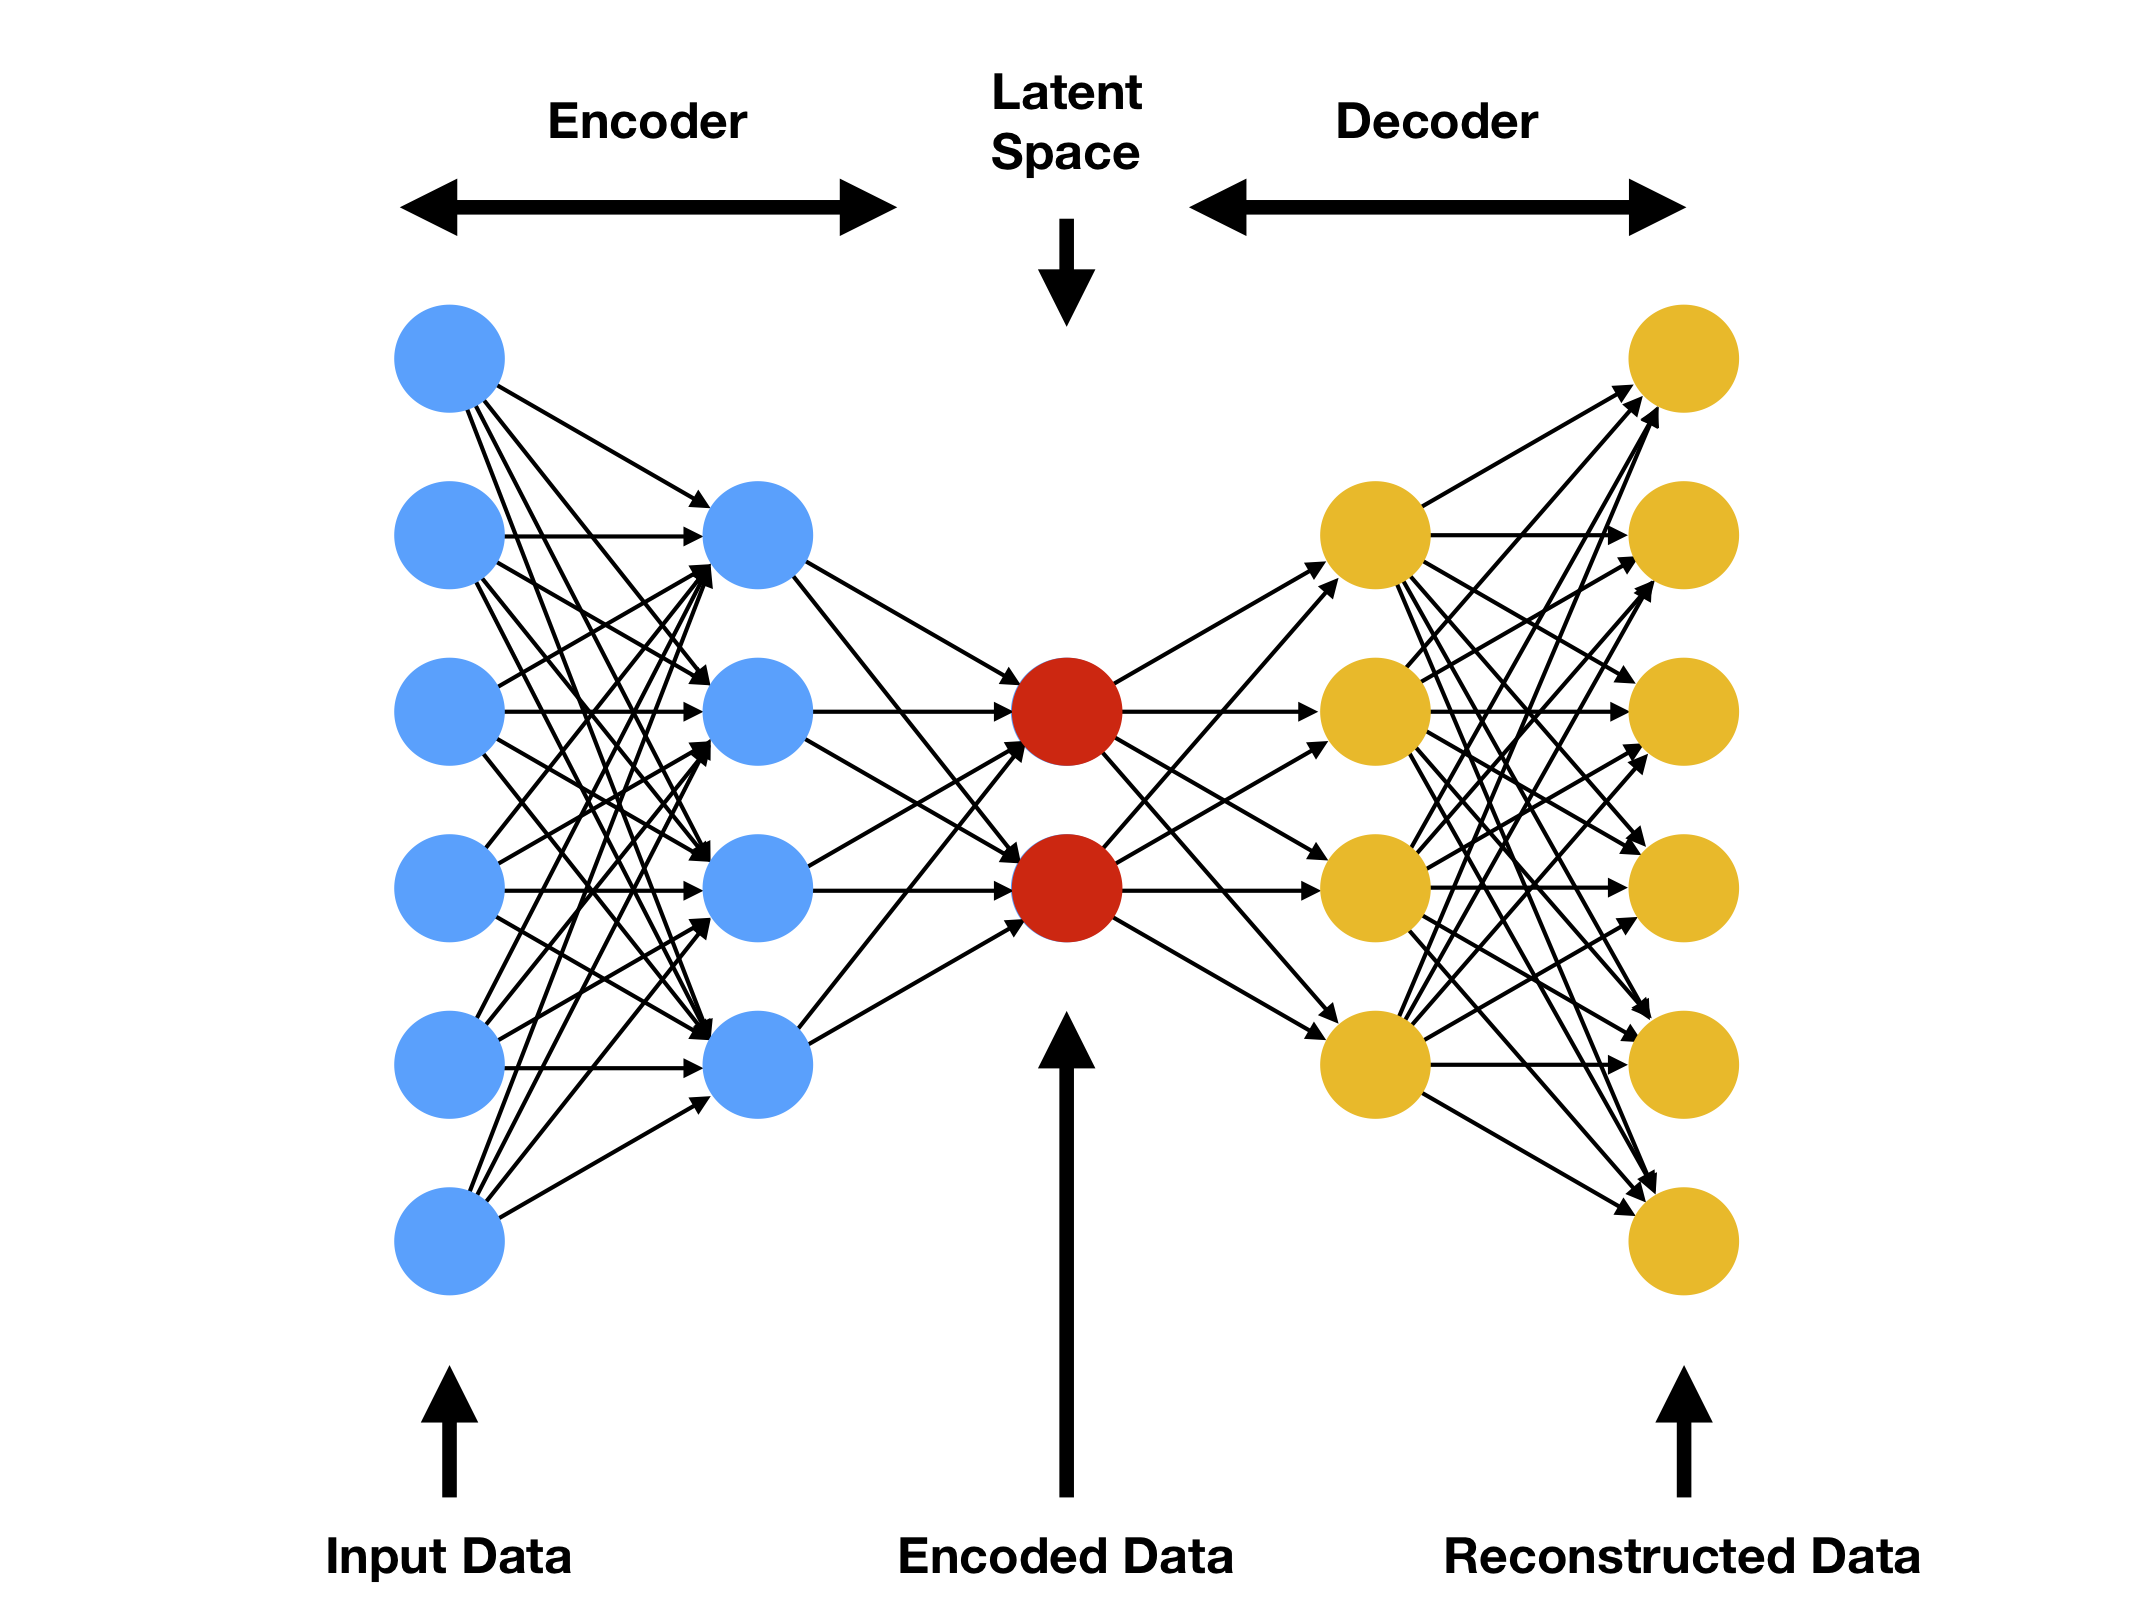
\includegraphics[width=.9\linewidth]{../resources/autoencoder.png}
\caption{The Autoencoder Structure}
\end{figure}
\end{frame}

\begin{frame}[label={sec:orge622e24}]{Representation Learning}
\begin{block}{Overview}
\begin{itemize}
\item Representation Learning is highly related to Dimensionality reduction.
\item Important to notice a good dimensionality reduction does not
necessarily learn a good representation and the opposite is also
true
\item Autoencoders are a "neutral" technique that gives a lot of
flexibility during training and enables to have more control on
different tradeoffs that are intrinsic of the problem
(i.e. dimensionality reduction vs representation learning)
\end{itemize}
\end{block}
\end{frame}

\begin{frame}[label={sec:org1735c55}]{Why create low dimensional latent space for DRL?}
\begin{block}{DARLA (DisentAngled Representation Learning Agent)}
\begin{itemize}
\item It shows that all DRL techniques  (implicitly) maps
the high dimensional state-space to a low dimensional state-space
and then maps this low dimensional state-space to the action space.
\item Therefore, we want to remove this concern from the DRL. We also want to do
this because we do not want the representation to be biased by the
DRL objective (which, in a nutshell, maximizes the rewards)
\end{itemize}
\end{block}
\end{frame}

\begin{frame}[label={sec:org961844b}]{MDPs Generalization}
\begin{block}{What is it?}
\begin{itemize}
\item it is the concept that exists only one natural world and we can sample MDPs
from it.
\item Each MDP will have the same action space. (If this does not apply,
it close to impossible to have transfer)
\item Different State spaces but some structural similarity
(i.e. isomorphisms)
\item so if we want to generalize we need to be able to have the same
representation for different MDPs
\item In order word, generalization in this context means be able to find the
common state space between MDPs (this must exists since we assumed
that we are sampling these MDPs from one single "natural world")
\end{itemize}
\end{block}
\end{frame}

\begin{frame}[label={sec:org433e658}]{Disentangled Representation?}
\begin{block}<1->{Definition}
There is not yet a definition on which the community agrees upon.
The best and the most formal attempt was done in Towards a definition of
disentangled representations. (exploiting concept of physics and group
theory)
\end{block}
\begin{block}<2->{In nutshell (quoting directly)}
Intuitevely, we define a vector representation as disentangled, if it
can be decomposed into a number of subspaces,each one of which is
compatible with, and can be transformed independently by a unique
symmetry transformation
\end{block}
\end{frame}

\begin{frame}[label={sec:orgda38cbd}]{Still not clear?}
Let's say we want to present an environment that has only a solid
and this solid has a colour and a position.
Ideally, we want to have a 3D vector where one dimension represents the
shape one the position and one the colour. This, in a superficial point
of view, is a disentangled representation.
\end{frame}

\begin{frame}[label={sec:org312001e}]{Examples of Entangled vs Disentangled representations}
\begin{center}
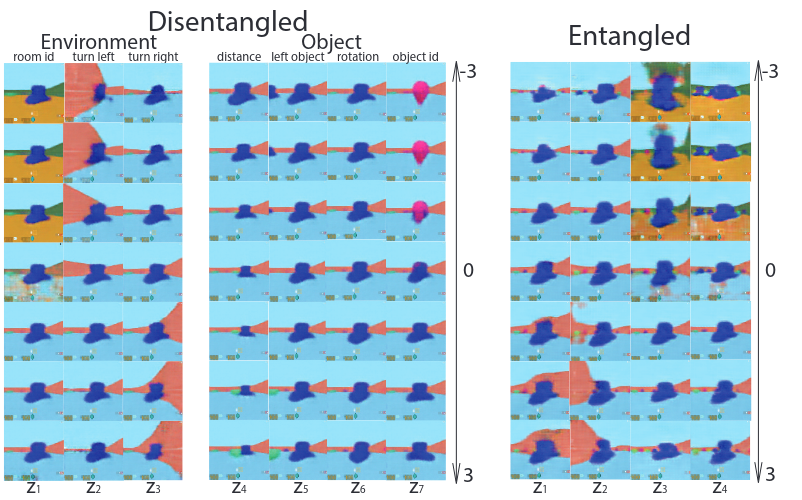
\includegraphics[width=.9\linewidth]{/home/vimmoos/thesis/resources/dis_vs_ent.png}
\end{center}
\end{frame}

\begin{frame}[label={sec:org60a2e7a}]{But why Disentangled representations?}
\begin{block}<1->{}
Also here the literature is not clear. There are a lot of papers which
shows that having such a representation has the following benefits on DRL
\begin{itemize}
\item increase the sample-efficiency
\item decrease the sensitivity to nuisance variables
(i.e. variables that are not too important for the decision process)
\item Better performance in terms of generalization
\end{itemize}
\end{block}
\begin{block}<2->{}
Formally though, there is no theory of why is the case, a good starting point is the paper Are Disentangled Representations Helpful for
Abstract Visual Reasoning?
Here they show experimentally (once again) that having such a representation
results in the aforementioned properties
\end{block}
\end{frame}
\begin{frame}[label={sec:org44e4149}]{Interesting point (2022 survey)}
\begin{center}
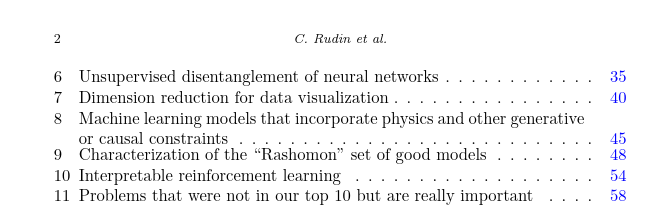
\includegraphics[width=.9\linewidth]{/home/vimmoos/thesis/resources/problems.png}
\end{center}
\end{frame}

\begin{frame}[label={sec:org7be4c23}]{What we will do in the thesis?}
\begin{block}<1->{}
We want to see whether these experimental gains also translates to
harder and more complex environment
\end{block}
\begin{block}<2->{}
if that will be the case we also want to address whether we can
generalize in a zero-shot transfer situation
\end{block}
\begin{block}<3->{}
The architectures we want to test are:
\begin{itemize}
\item Sparse Autoencoders (already implemented)
\item Variational Autoencoders (already implemented)
\item \(\beta\) Variational Autoencoders
\item Mutual information Variational Autoencoders
\item Adversarial Variational Bayes (already implemented)
\end{itemize}
\end{block}
\end{frame}
\begin{frame}[label={sec:org0444cdf}]{Ideas for future research}
\begin{block}{}
\begin{itemize}
\item test other Disentanglement AE/GAN architectures (e.g. FactorVAE,CasualVAE,DreamingVAE).
\item explicitly focus on transfer (maybe with fine-tuning instead of
zero-shot)
\item test different DRL algorithm to see how this impact the performance
\item test different method of training the AE (for example on-line, see
active perceptions frameworks and/or active learning currently in
development by Microsoft research closely followed by  Yoshua
Bengio)
\item In general, the idea of representation learning + DRL seems to be
a really interesting and not fully explored path. (see The Consciusness
Prior by Yoshua Bengio)
\end{itemize}
\end{block}
\end{frame}

\begin{frame}[label={sec:org2844dc9}]{Reference}
For more reference and in-depth explanation of the research process
see \url{https://172.104.159.41/thesis/summary.html} which is constantly
update with every single step we are taking and the
motivation/explanation of why we are taking such steps
\end{frame}
\end{document}
